\chapter{Conclusions}
\label{chap:conclusions}

The following section present the conclusion where the impact of the flying height and users population in a \gls{UAV}-aided network
is investigated by examining electromagnetic exposure and power consumption. Also, an optimization techniques towards both evaluation 
parameters have been applied and two different antenna types have been considered.
All conclusions are based on the default configuration with a flying height of 100 metres and 224 active users to cover.
The other parameters are described in table \ref{table:defaultconf}.

\section{Conclusion}

%How can a UABS network be optimized to minimize global exposure or overall power consumption? 
Literature showed that a network can be optimized towards either the power consumption of the entire network 
or the electromagnetic exposure of the average user using a fitness function. This is because the power required to activate a new 
base station is much higher then for raising the electromagnetic radiation and therefore increasing its range \cite{J1}.
The fitness function was originally applied for fixed transmission towers but can also be used 
for \gls{UABS}s as this research shows.
However, the fitness function should be used with care considering that \gls{UABS}s can be placed anywhere as opposed to 
the transmission towers from \cite{J1} who have a predetermined position.  
For default networks, the electromagnetic field radiation from a
power consumption optimized network can be reduce up to 23\% for \gls{isotropicradiator}s and 30\% for microstrip patch antenna 
by optimizing towards electromagnetic exposure. Doing so, decreases the range of the \gls{UABS} and much more \gls{UABS}s will be needed. 
Therefore, exposure optimized networks will, on average, use 18 drones more than power consumption optimized networks
and requires therefore 5 $W$ more energy.
A power consumption optimized network on the other hand will try to limit the number of drones 
in order to save energy.
 So as a rule of thumb: an exposure optimized network will result in a lot of low powered devices (increasing the overall power consumption)
while a power consumption optimized network results in a few high powered devices (increasing the exposure of the average user).
The authors from \cite{J17_kuehn2019modelling} confirm this by stating that smaller cells will reduce electromagnetic radiation. 
If the goal is to remain in the air for a longer period of time, an exposure optimized network is recommended because the power consumption of 
an individual \gls{UABS} is lower.
On the other hand, a power consumption optimized network is cheaper because less drones are involved.
Moreover, the results show that the electromagnetic radiation in a power consumption optimized network (with high powered \gls{UABS}s)
is far below the thresholds enforced by the Flemish government with more than one millionth of the maximal allowed whole body \gls{SAR}.

\definecolor{c_myuabs}{HTML}{A9C6FC}
\definecolor{c_otheruabs}{HTML}{7A4655}
\definecolor{c_myue}{HTML}{90AF74}
\definecolor{c_otherue}{HTML}{F4A259}

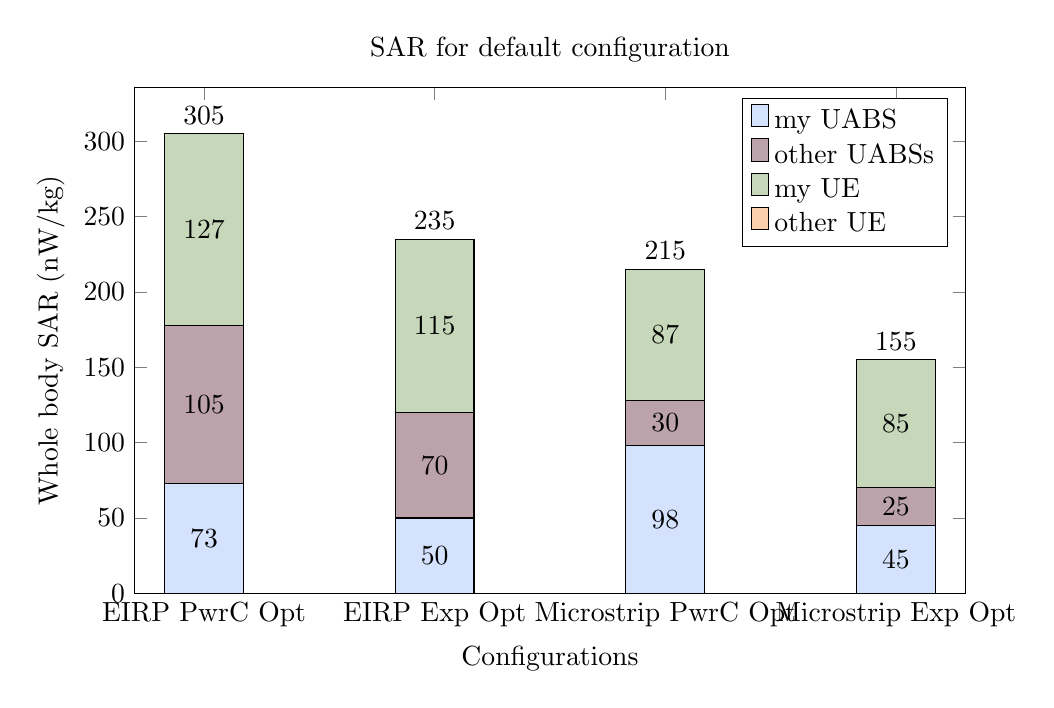
\begin{tikzpicture}
\pgfplotsset{
        show sum on top/.style={
            /pgfplots/scatter/@post marker code/.append code={%
                \node[
                    at={(normalized axis cs:%
                            \pgfkeysvalueof{/data point/x},%
                            \pgfkeysvalueof{/data point/y})%
                    },
                    anchor=south,
                ]
                {\pgfmathprintnumber{\pgfkeysvalueof{/data point/y}}};
            },
        },
    }
  \begin{axis}[
    title={SAR for default configuration},
    ylabel={Whole body SAR (nW/kg)},
    xlabel={Configurations},
    height=8cm, width=\textwidth,
    legend cell align={left},
    ybar stacked, ymin=0,  
    bar width=10mm,
    %symbolic x coords={a,b,c,d},
    symbolic x coords={EIRP PwrC Opt, EIRP Exp Opt, Microstrip PwrC Opt, Microstrip Exp Opt},
    xtick=data,
    nodes near coords, 
    nodes near coords align={anchor=center},%Move values in bar
    every node near coord/.style={
    },
  ]
  %myUABS
  \addplot [fill=c_myuabs!50] coordinates {
({EIRP PwrC Opt},73)
({EIRP Exp Opt},50)
({Microstrip PwrC Opt},98)
({Microstrip Exp Opt},45)};
  %other uabs
  \addplot [fill=c_otheruabs!50,text=black] coordinates {
({EIRP PwrC Opt},105)
({EIRP Exp Opt},70)
({Microstrip PwrC Opt},30)
({Microstrip Exp Opt},25)
};
%myue
  \addplot [fill=c_myue!50,show sum on top] coordinates {
({EIRP PwrC Opt},127)
({EIRP Exp Opt},115)
({Microstrip PwrC Opt},87)
({Microstrip Exp Opt},85)
};
%other ue
  \addplot [fill=c_otherue!50,show sum on top] coordinates {
({EIRP PwrC Opt},0)
({EIRP Exp Opt},0)
({Microstrip PwrC Opt},0)
({Microstrip Exp Opt},0)
};
  \legend{my UABS,other UABSs,my UE,other UE}
\end{axis}
\end{tikzpicture}


%	How does the network behave differently after the introduction of a realistic antenna?
A directional microstrip patch antenna is introduced because it gives several advantages compared to omnidirectional antennae.
Directional antennae are able to focus their energy there where it is needed, namely towards the ground. Microstrip patch antennae 
further benefit from their thin and lightweight design. The performance 
of this directional microstrip patch antenna has been compared to a 
fictional \gls{isotropicradiator}.
This \gls{isotropicradiator} has higher exposure and coverage for less power compared to an microstrip patch antennae.
For a default network, a microstrip patch antenna can reduce between 30\% and 34\% electromagnetic exposure 
from an \gls{isotropicradiator}. Doing so will increase the power consumption with 11 $W$.
The fact that an \gls{isotropicradiator} has higher electromagnetic exposure for less power  is due to the absence of 
attenuation and can hypothetically be compared to an antenna with a very big aperture angle.
A microstrip patch antenna with a more limited aperture angle of \ang{90} requires more resources but 
causes less sideways radiation. So the exposure from other \gls{UABS}s will also be less.

\begin{figure}[hb!]
\centering
  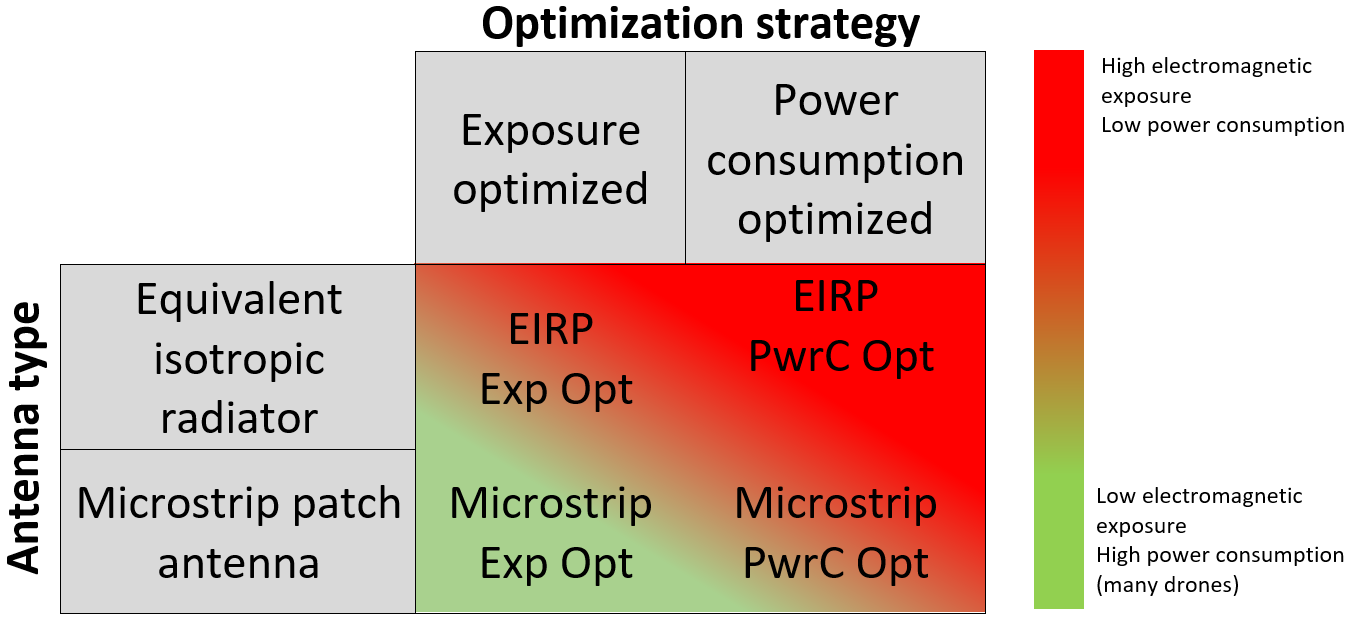
\includegraphics[width=0.9\textwidth]{../images/fourCasesMatrixSol.png}
  \caption{Matrix with the four possible configurations, colour-coded based on the results.}
  \label{fig:resultIllustration}
\end{figure}

Figure \ref{fig:resultIllustration} shows an overview based on the results from the two optimization strategies and the two types of antenna.
Remarkable is that an \gls{EIRP} exposure optimized network behaves very similar to a microstrip power consumption optimized network.
Therefore, the microstrip patch antenna in a power consumption optimized network is recommended. 
The microstrip patch antenna will generate less electromagnetic radiation by design and
 the power consumption optimization reduces the number of required drones and power. A microstrip patch antenna with an aperture 
 angle of \ang{90} is considered as a good solution but if budget is more limited, an antenna with a larger aperture angle 
 would further reduce cost without interfering with the Flemish legislation regarding electromagnetic exposure.


%What is the contribution of each source towards the total electromagnetic exposure?
Figure \ref{fig:pie} gives
an overview of the contribution of \gls{SAR} in percentage to the total 
exposure for a default network. The values have been averaged over all four possible configurations. 
The user's main sources of exposure is clearly the user's own device which contributes 52\% of the total experienced exposure.
A conclusion that was also made by the authors of \cite{J17_kuehn2019modelling}
where a 5G network is simulated and by the authors from  \cite{J10.1.1} 
where a \gls{GSM} and \gls{UMTS} network is simulated. However, in \cite{J10.1.1} is also concluded that,
thanks to power control, the electromagnetic radiation from the mobile phone 
comes really close to the exposure from the \gls{UABS}. 
Also this is confirmed by the results. Figure \ref{fig:pie} shows that the electromagnetic exposure 
from all \gls{UABS}s together covers the remaining 48\% of which 15 \% is from the serving UABS. 
The electromagnetic
 exposure from devices belonging to other people can be ignored compared to the much higher electromagnetic exposure from the other sources
 and contributes only 0.0001\%. It is important to notice that a rather low \gls{pusch} value is used in equation \ref{eq:powerUE} for determining the 
 \gls{UL} radiation and it is believed that a higher value will have a major effect on the \gls{SAR} from the user's own 
 device but also from neighbouring devices.

\def\angle{0}
\def\radius{3}
\def\cyclelist{{"c_myue","c_otheruabs","c_myuabs","c_otherue"}}
\newcount\cyclecount \cyclecount=-1
\newcount\ind \ind=-1
\begin{figure}
\centering
 \resizebox {!} {6cm} {
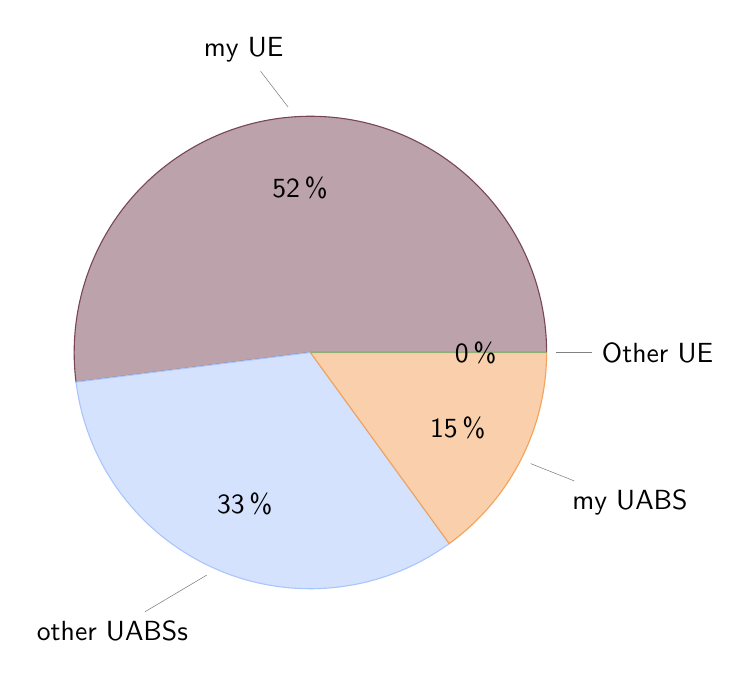
\begin{tikzpicture}[nodes = {font=\sffamily}]
  \foreach \percent/\name in {
      52/ my UE,
      33/ other UABSs,
      15/ my UABS,
      0/ Other UE
    } {
      \ifx\percent\empty\else               % If \percent is empty, do nothing
        \global\advance\cyclecount by 1     % Advance cyclecount
        \global\advance\ind by 1            % Advance list index
        \ifnum3<\cyclecount                 % If cyclecount is larger than list
          \global\cyclecount=0              %   reset cyclecount and
          \global\ind=0                     %   reset list index
        \fi
        \pgfmathparse{\cyclelist[\the\ind]} % Get color from cycle list
        \edef\color{\pgfmathresult}         %   and store as \color
        % Draw angle and set labels
        \draw[fill={\color!50},draw={\color}] (0,0) -- (\angle:\radius)
          arc (\angle:\angle+\percent*3.6:\radius) -- cycle;
        \node at (\angle+0.5*\percent*3.6:0.7*\radius) {\percent\,\%};
        \node[pin=\angle+0.5*\percent*3.6:\name]
          at (\angle+0.5*\percent*3.6:\radius) {};
        \pgfmathparse{\angle+\percent*3.6}  % Advance angle
        \xdef\angle{\pgfmathresult}         %   and store in \angle
      \fi
    };
\end{tikzpicture}
 }
\caption{Contribution from each source towards the total SAR that is experienced by the weighted average user. 
The percentages are averaged over the four 
considered configurations.}
\label{fig:pie}
\end{figure}

%How does the \gls{UABS} flying height and number of users influence electromagnetic exposure and power consumption?
As last, the results confirm that the flying height and population size has a major influence on electromagnetic exposure and 
power consumption. It becomes clear that more \gls{UABS}s are required when the population size increases. 
This comes with a higher power 
consumption and electromagnetic exposure. When the population increases from 50 to 600 users, 
the electromagnetic radiation increases between 80 and 130 $mV/m$ depending
on the configuration. The power consumption increases with 110 $W$ for all configurations. 
The main source that is influenced by the number of users is the \gls{SAR} from other UABSs with an increase between 1 and 3 $\mu W/kg$, depending on 
the configuration.
Further, increasing the flying altitude has a positive influence on the number of required drones which on his 
turn has a positive influence on power consumption. Increasing the flying altitude from 50 m to 200 m, decreases the number 
of required drones around 59\%. This decrease in number of \gls{UABS}s was also concluded in \cite{J2}.
Also authors from \cite{J17_kuehn2019modelling} made the conclusion that reduced path loss decreases electromagnetic exposure.
The electromagnetic radiation from the \gls{UABS}s does not change for flying altitudes between 80 and 200 metres. Most 
\gls{UABS}s are in \gls{LOS} and no more power will be used thanks to power control.
However, the electromagnetic radiation from the user's own device does increase in order to reach the high flying drones.
Around 80 metres, the exposure from the  user's device surpasses the exposure from the serving \gls{UABS}.
When more \gls{UABS}s are available in the network, electromagnetic exposure from other \gls{UABS} will increase as well 
because more \gls{UABS}s come into \gls{LOS}. Raising the flying altitude from 50 to 200 m will increase the \gls{SAR} from other 
\gls{UABS}s between 49 and 46 times when using a \gls{EIRP} antenna and between 70 and 85 times when using a for microstrip patch antenna.
It is therefore concluded that raising the flying height has a positive but is not unlimited.
When also considering the results from \cite{U1} where a flying altitude of  
80 metres is suggested for an optimal access and backhaul connectivity, a flying height 
of 80 metres is also here proposed for the city centre of Ghent.

\section{Summary}
The microstrip patch antenna with an aperture angle of \ang{90} is a suitable starting point for an antenna. 
This directional antenna focusses electromagnetic radiation where it is needed. Unwanted sideways radiation 
is therefore reduced by design.
The sufficiently large aperture angle covers enough users. The antenna is recommended the be deployed in a power consumption 
optimized network since less drones are required and therefore also less expensive.
The optimal flying height for the city center of Ghent is believed to be situated at 80 metres since lower flying heights require much more \gls{UABS} and
higher flying heights has a negative influence on the electromagnetic exposure.  

\section{Future work}

Despite the fact the many parameters has been examined, still some parameters require further investigations.
The \gls{pusch} value defines the minimal required signal strength received by the \gls{UABS} and still need to be evaluated
for different values. Also, the exposure caused by backhaul links has not been evaluated yet.

The chosen microstrip patch antenna is solely based on literature and performing an excessive research to various 
types of radiation patterns is outside the scope of this master dissertation. It is expected that the radiation can 
further be improved by using microstrip patch antennae in more complex array-configurations. 

The tool provide support for any possible radiation pattern and applies this to any \gls{UABS}.
However, despite some minor changes, each \gls{UABS} can has it's custom radiation pattern which makes 
3D beamforming possible. Therefore, electromagnetic exposure can be determined for base stations where MiMo
and massive MiMo is in use.

Also, the tool makes use of an \gls{exact algorithm}. Despite the fact that several  
tactics have been introduced to improve performance, large populations still cause long runtimes. It might be useful 
to reduce the quality of the result in order to improve performance. Mozafari et al. discusses in \cite{U3} several 
other approaches besides \gls{exact algorithm}s like heuristic methods, machine learning and so on.